\documentclass[11pt]{article}

\usepackage[margin=1in]{geometry}
\usepackage{amsmath,amssymb,mathtools}
\usepackage{booktabs}
\usepackage{array}
\usepackage{graphicx}
\usepackage{hyperref}

\title{Kernel-Induced Operator Architecture and the Emergence of a Transverse Spectral Band on Discrete Substrates}
\author{Tomislav Rupi\'c}
\date{March 10, 2026}

\begin{document}
\maketitle

\begin{abstract}
This paper documents the current committed numerical results in the HAOS-IIP repository at the level of operator construction and spectrum. A Gaussian interaction kernel defines a weighted discrete substrate from which two operator lifts are studied: a node operator for the scalar sector and an edge or Hodge operator for the vector-sector candidate. On cubic graphs, the kernel-induced difference operator converges to the continuum Laplacian after discrete second-moment normalization. On periodic edge complexes, the restricted transverse operator $T = d_1^* d_1 \vert_{\ker(d_0^*) \cap (\mathcal{H}^1)^\perp}$ exhibits a descending low spectrum, decreasing inverse participation ratio, and partial $n^2$ spectral collapse across lattice sizes and defect branches. The results are presented strictly as operator-level numerical evidence. No claim is made for Maxwell dynamics, gauge theory, or physical photon modes.
\end{abstract}

\section{Introduction}
The numerical program documented here asks a narrow question: can multiple continuum operator sectors emerge from the same discrete interaction substrate? The repository addresses that question by fixing a single kernel-defined weighted graph and then constructing different operator lifts on top of it. The resulting pipeline is
\begin{equation}
\text{kernel} \to \text{operators} \to \text{spectrum}.
\end{equation}
The scalar branch is probed through a graph Laplacian limit, and the edge branch is probed through a discrete Hodge operator together with a restricted transverse sector. Discrete Hodge Laplacians generalize graph Laplacians to higher-degree objects and encode gradient, divergence, and curl structure on discrete complexes.\footnote{Background overview: \url{https://www.emergentmind.com/topics/discrete-hodge-laplacians}} The present paper does not broaden the theory. It documents committed experiments already in the repository and reports only operator-level numerical conclusions.

The current computational narrative is:
\begin{equation}
\text{kernel-defined substrate}
\to
\text{scalar Laplacian limit}
\to
\text{edge/Hodge sector}
\to
\text{restricted transverse spectrum}.
\end{equation}
The main objective of this paper is to summarize the numerical evidence for that chain in a form suitable for a computational physics report.

\section{Kernel-Defined Substrate}
The common substrate is generated by the Gaussian interaction kernel
\begin{equation}
A_{ij} = \exp\!\left(-\frac{|x_i-x_j|^2}{2\varepsilon_k}\right),
\end{equation}
with embedded nodes $x_i \in \mathbb{R}^3$. For the scalar convergence experiments, the cubic scan uses lattice spacing $h$ and the kernel-width scaling
\begin{equation}
\varepsilon_k = c_\varepsilon h^2,
\qquad
c_\varepsilon \in \{0.5, 1.0, 2.0\}.
\end{equation}
This keeps the kernel in a local regime as the grid is refined. The weighted adjacency matrix is denoted by $A$ or $W$, with degree matrix
\begin{equation}
D_{ii} = \sum_j A_{ij},
\end{equation}
and graph Laplacian
\begin{equation}
L = D - A.
\end{equation}
For the edge-sector experiments, the same cubic substrate is lifted to a periodic cell complex with oriented edges and faces. The operator definitions are held fixed throughout the defect and scaling scans; only the substrate topology or local defect structure is changed.

A key technical point from the committed convergence experiment is that the raw graph object $L = D-A$ is not compared directly to $\Delta$. The correct induced continuum operator is the normalized difference operator
\begin{equation}
\widehat{L}_h = -\frac{2}{\mu_2 h^2}L,
\end{equation}
where $\mu_2$ is the discrete second moment of the actual kernel stencil. This normalization is what produces the observed Laplacian limit.

\section{Scalar Operator and Laplacian Limit}
The scalar experiment \texttt{Kernel\_Laplacian\_Convergence\_v1} tests whether the kernel-induced operator converges to the continuum Laplacian on cubic grids with $n = 9, 11, 13, 17, 21$. Three analytic test functions are used:
\begin{align}
 f_1(x,y,z) &= x^2+y^2+z^2, \\
 f_2(x,y,z) &= \sin(\pi x)\sin(\pi y)\sin(\pi z), \\
 f_3(x,y,z) &= \exp\!\left(-(x^2+y^2+z^2)\right).
\end{align}
Their continuous Laplacians are known exactly, so the interior operator error
\begin{equation}
\|\widehat{L}_h f - \Delta f\|_2
\end{equation}
can be measured directly.

The quadratic test is reproduced to machine precision on interior nodes, which is the expected behavior for a second-order Laplacian approximation on a regular stencil. For the trigonometric test, the fitted convergence orders are
\begin{equation}
1.9825 \; (c_\varepsilon=0.5),
\qquad
1.8579 \; (c_\varepsilon=1.0),
\qquad
1.3770 \; (c_\varepsilon=2.0).
\end{equation}
For the Gaussian test, the corresponding orders are
\begin{equation}
1.8035,
\qquad
1.2495,
\qquad
0.3316.
\end{equation}
The weaker performance at $c_\varepsilon=2.0$ is consistent with the kernel becoming too broad relative to the grid spacing, so the operator is less local at finite resolution.

\begin{table}[t]
\centering
\begin{tabular}{lccc}
\toprule
Test function & $c_\varepsilon=0.5$ & $c_\varepsilon=1.0$ & $c_\varepsilon=2.0$ \\
\midrule
$f_1 = x^2+y^2+z^2$ & machine precision & machine precision & machine precision \\
$f_2 = \sin(\pi x)\sin(\pi y)\sin(\pi z)$ & 1.9825 & 1.8579 & 1.3770 \\
$f_3 = e^{-(x^2+y^2+z^2)}$ & 1.8035 & 1.2495 & 0.3316 \\
\bottomrule
\end{tabular}
\caption{Measured convergence orders for the normalized kernel-induced scalar operator. The local-kernel regime $\varepsilon_k \sim h^2$ with $c_\varepsilon \le 1$ gives the cleanest Laplacian behavior.}
\label{tab:scalar-convergence}
\end{table}

\begin{figure}[t]
\centering
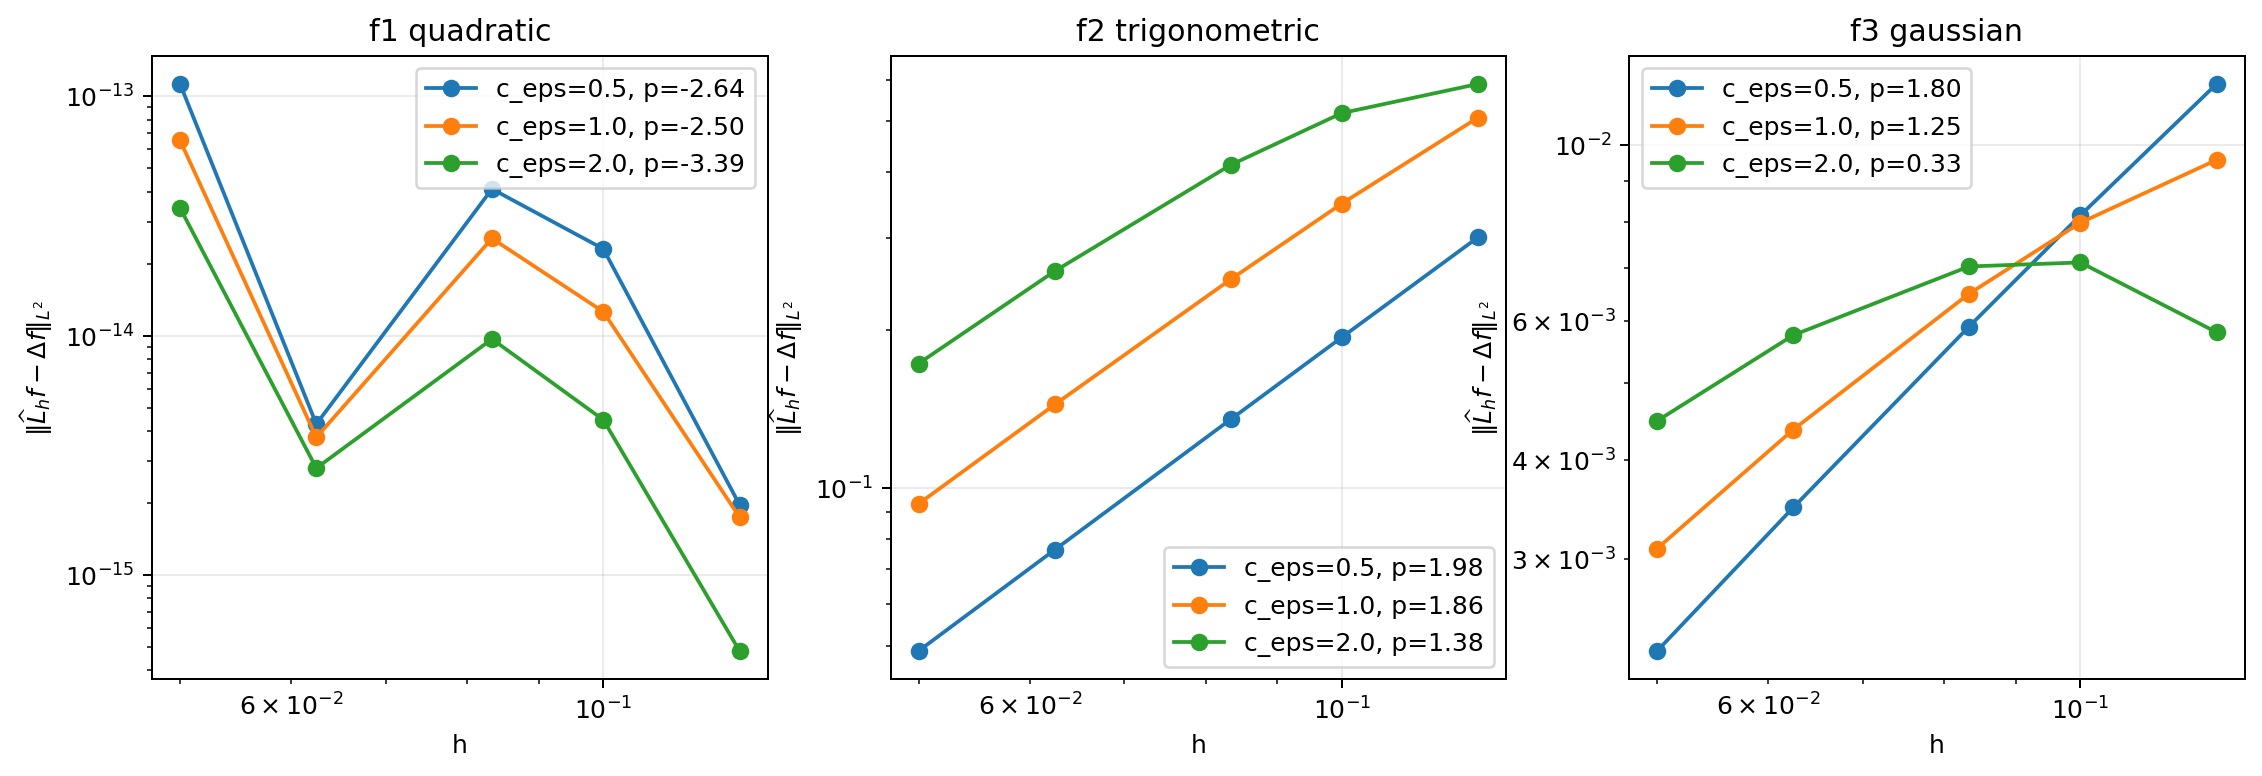
\includegraphics[width=0.48\linewidth]{../plots/20260310_111522_operator_error_vs_h.png}
\hfill
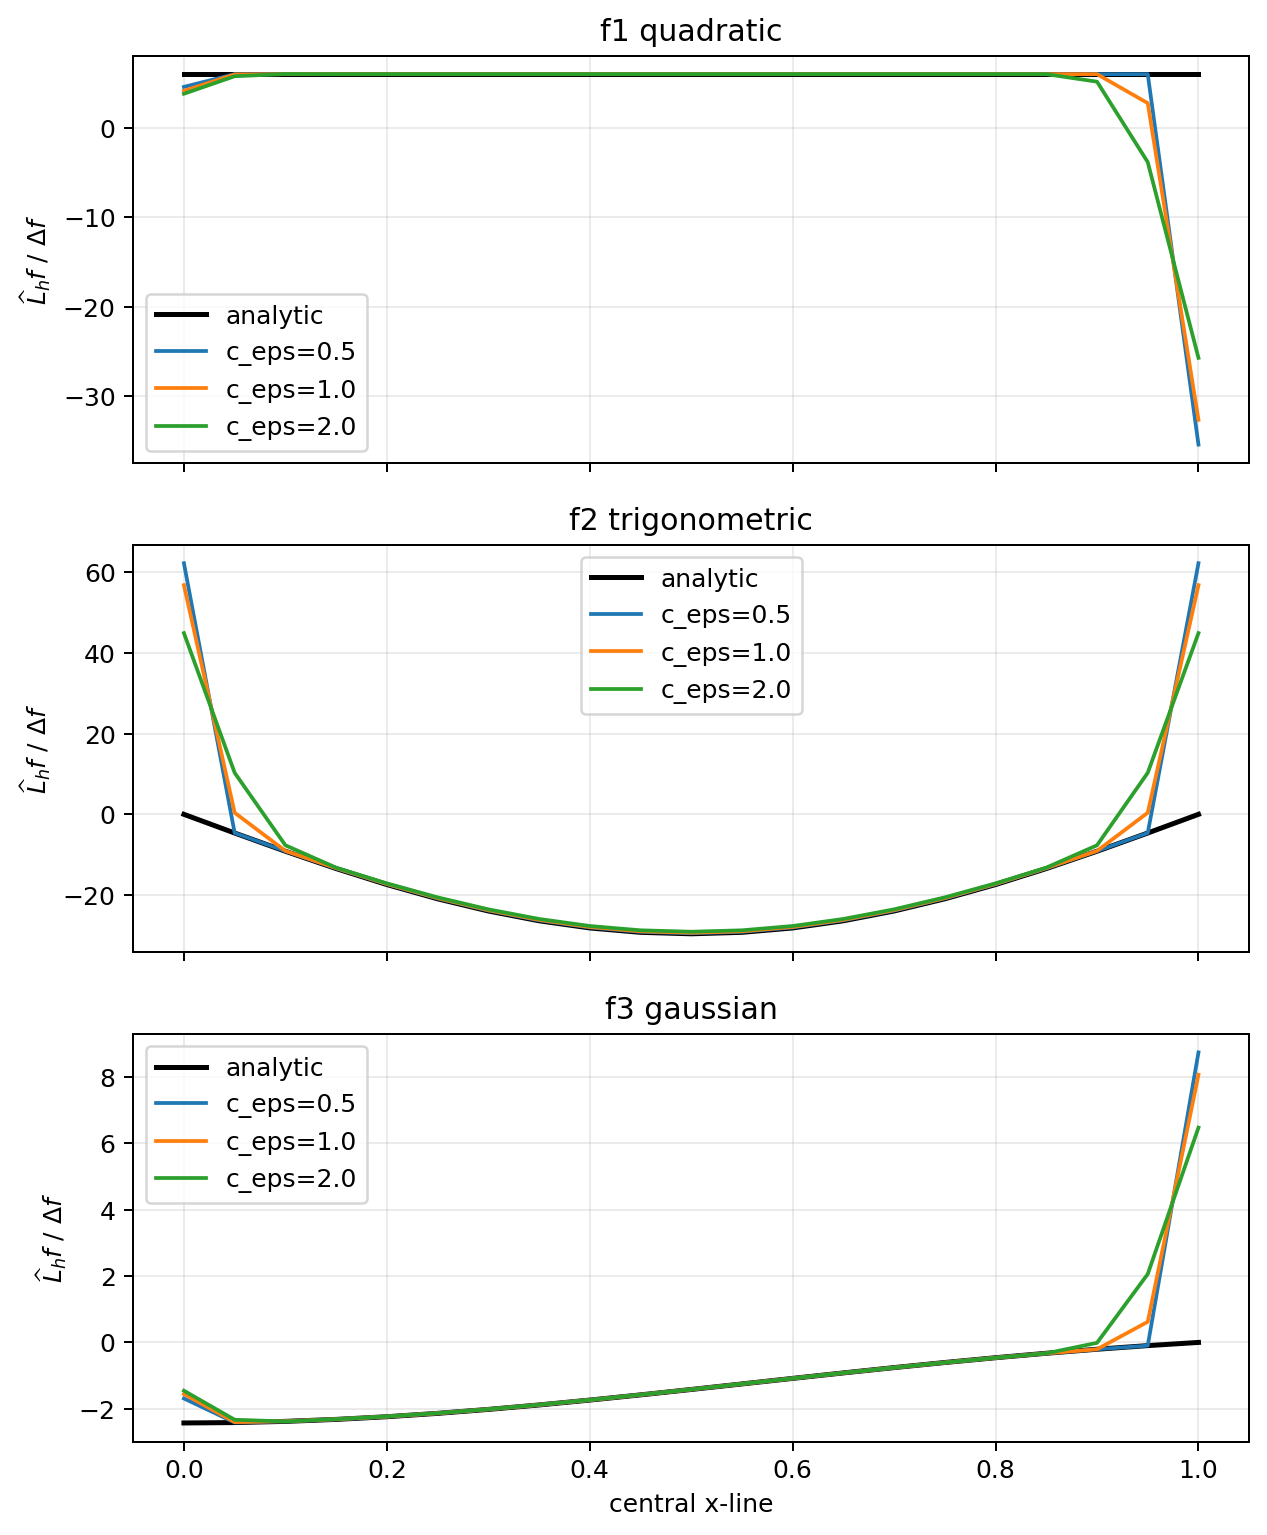
\includegraphics[width=0.48\linewidth]{../plots/20260310_111522_operator_profiles.png}
\caption{Committed plots from \texttt{Kernel\_Laplacian\_Convergence\_v1}. Left: operator error versus grid spacing for the three analytic tests and three kernel widths. Right: representative interior operator profiles compared with the analytic continuum Laplacian.}
\label{fig:scalar-convergence}
\end{figure}

Within the tested range, the scalar branch therefore supports the statement that the normalized kernel operator converges to the continuum Laplacian. This establishes the scalar sector used elsewhere in the repository.

\section{Edge Operator Architecture}
The edge-sector construction is built on oriented node-edge and face-edge incidence maps. With weighted differentials
\begin{equation}
 d_0 = W_1^{1/2} B_0,
 \qquad
 d_1 = W_2^{1/2} C,
\end{equation}
the edge or Hodge operator is
\begin{equation}
L_1 = d_0 d_0^* + d_1^* d_1.
\end{equation}
This operator acts on discrete $1$-forms supported on edges. The Hodge decomposition of edge space is
\begin{equation}
C^1 = \operatorname{im} d_0 \oplus \mathcal{H}^1 \oplus \operatorname{im} d_1^*,
\end{equation}
with exact, harmonic, and coexact components. Here
\begin{equation}
\mathcal{H}^1 = \ker(d_0^*) \cap \ker(d_1).
\end{equation}
The full $L_1$ spectrum is useful for exposing the entire Hodge structure, but the committed experiments show that the bottom of the unrestricted spectrum is naturally occupied by exact leakage or harmonic torus modes. The restricted transverse operator used for the later numerical tests is therefore
\begin{equation}
T = d_1^* d_1\big|_{\ker(d_0^*) \cap (\mathcal{H}^1)^\perp}.
\end{equation}
On this subspace, the exact and harmonic sectors are removed, so the remaining spectrum tests whether a genuinely coexact low branch exists.

\section{Initial Edge-Sector Diagnostics}
The first committed edge-sector diagnostic is the open-versus-periodic comparison in \texttt{Periodic\_Twisted\_L1\_Experiment\_v1}. On the open $n=5$ box, the lowest three edge modes are exactly gradient-like:
\begin{center}
\begin{tabular}{cccc}
\toprule
mode & eigenvalue & exact fraction & coexact fraction \\
\midrule
0 & 0.326713 & 1.000 & 0.000 \\
1 & 0.326713 & 1.000 & 0.000 \\
2 & 0.326713 & 1.000 & 0.000 \\
\bottomrule
\end{tabular}
\end{center}
This is the scalar-leakage baseline.

The same experiment on a periodic $n=5$ torus with trivial flux produces three exactly divergence-free and curl-free harmonic cycles at zero eigenvalue. With nontrivial twist $m=1$, those harmonic modes are lifted but remain largely non-exact; the lowest mode has eigenvalue $0.013057$ with exact fraction $0.025$ and divergence-free fraction $0.975$. This establishes that the edge operator supports genuine non-scalar structure once the topology is changed, but it also shows why topology control is needed: open-box modes are exact, while periodic modes mix harmonic torus cycles into the bottom of the spectrum.

\section{Defect Transverse Test}
The next committed step is \texttt{L1\_Defect\_Transverse\_Test\_v1}, which keeps the operator fixed and modifies only the substrate. Three branches are compared for $n = 6, 8, 10$:
\begin{enumerate}
\item baseline periodic torus,
\item single cubic puncture,
\item line defect.
\end{enumerate}
For each branch, the restricted transverse spectrum of $T$ is computed. The lowest restricted eigenvalues are:
\begin{table}[t]
\centering
\begin{tabular}{lccc}
\toprule
Branch & $n=6$ & $n=8$ & $n=10$ \\
\midrule
Baseline torus & 0.932912 & 0.563345 & 0.372535 \\
Puncture & 0.684887 & 0.441271 & 0.317111 \\
Line defect & 0.766501 & 0.514298 & 0.350303 \\
\bottomrule
\end{tabular}
\caption{Lowest restricted transverse eigenvalue from \texttt{L1\_Defect\_Transverse\_Test\_v1}. In all branches the floor decreases with lattice size, and both defect branches lie below the baseline torus at the same $n$.}
\label{tab:defect-floor}
\end{table}

\begin{figure}[t]
\centering
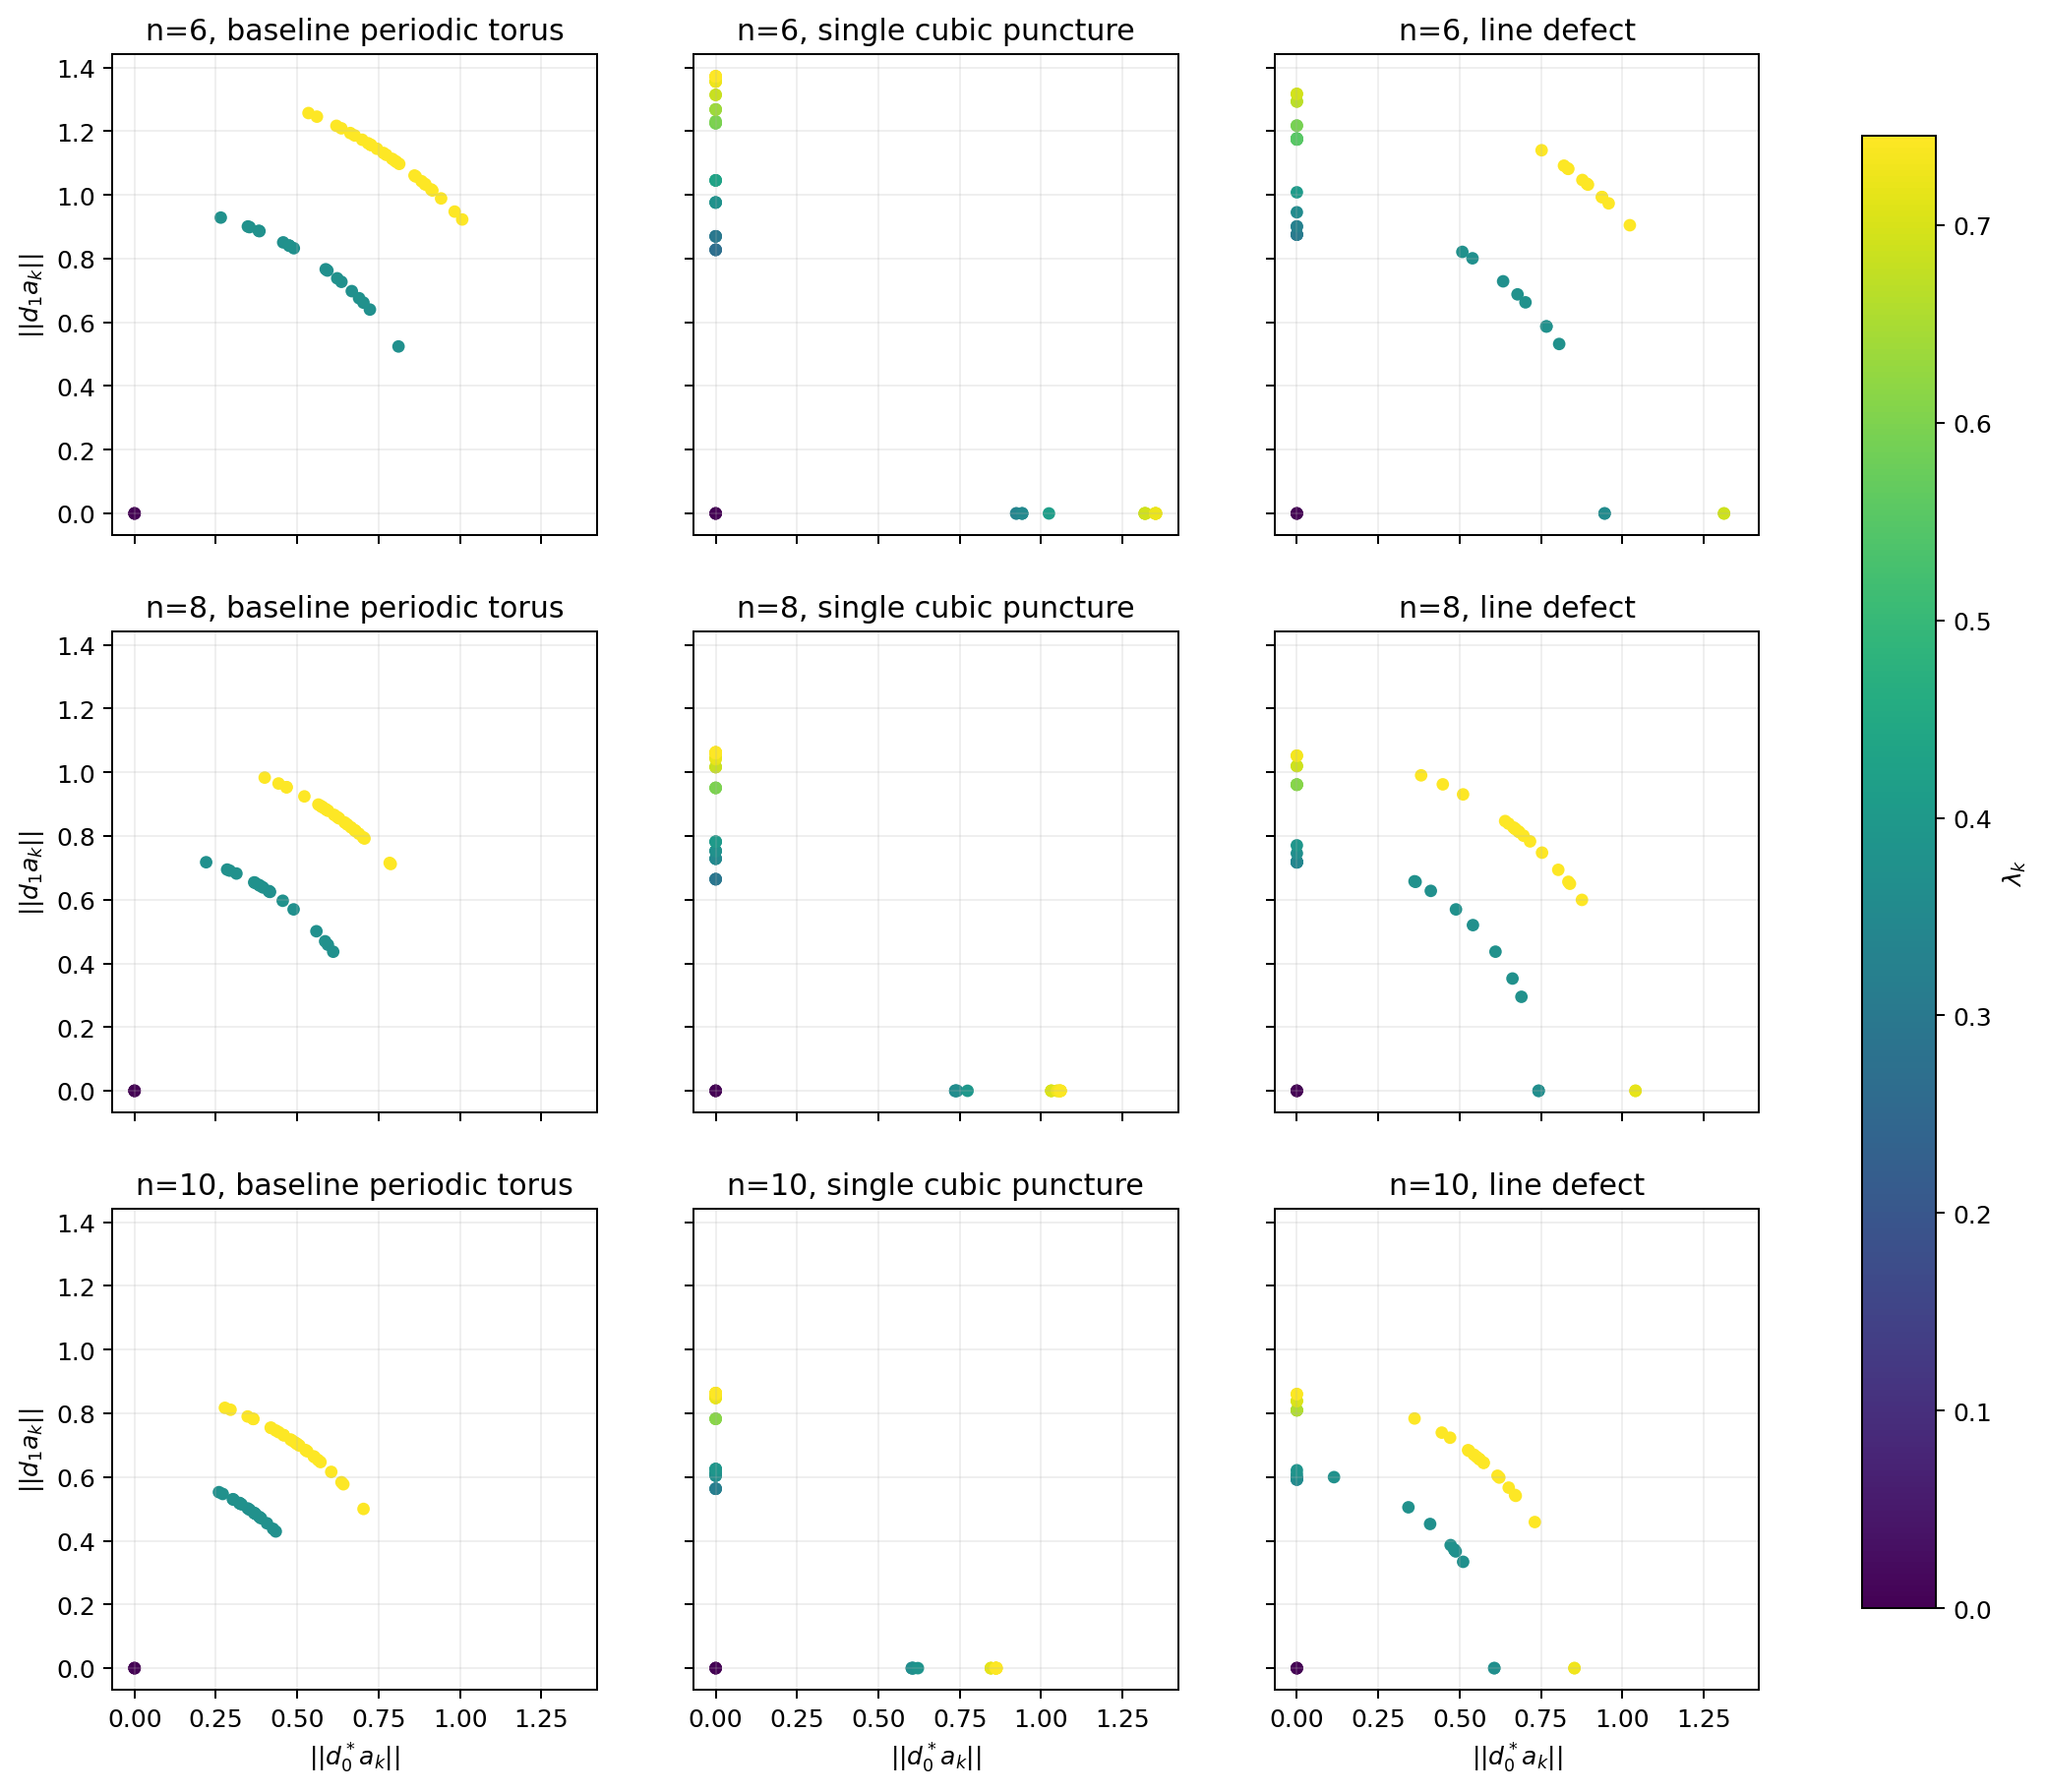
\includegraphics[width=0.32\linewidth]{../plots/20260310_130326_divergence_curl_phase.png}
\hfill
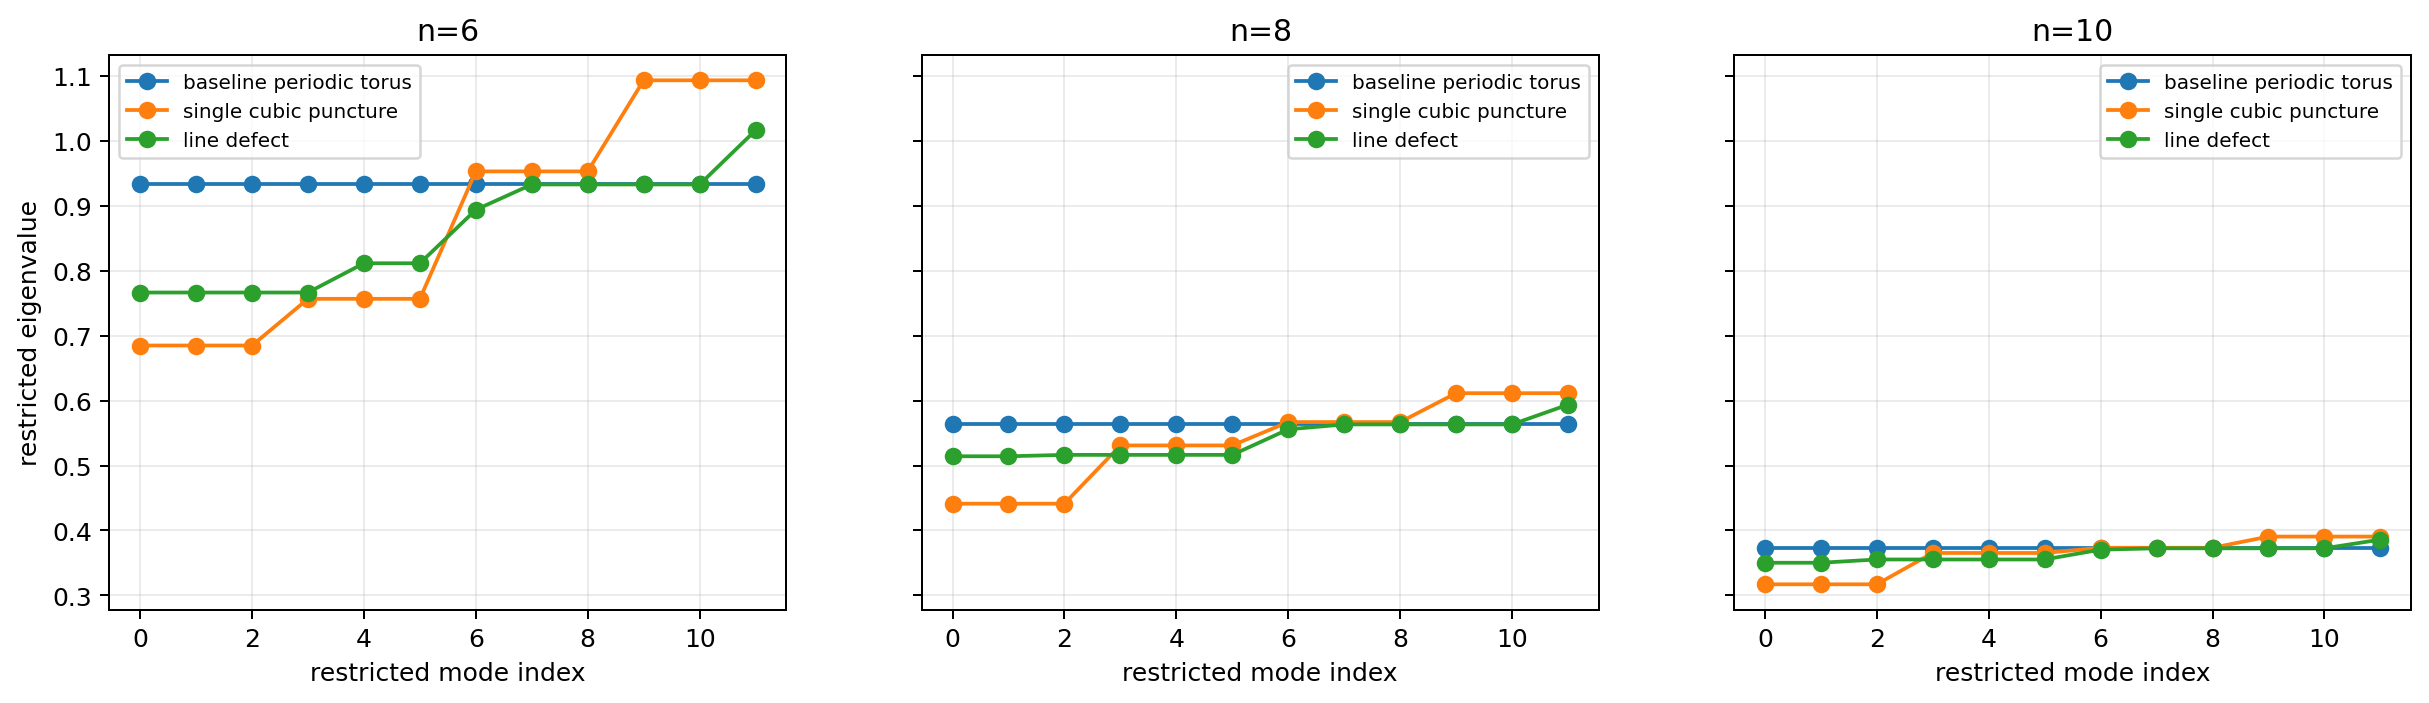
\includegraphics[width=0.32\linewidth]{../plots/20260310_130326_restricted_transverse_spectrum.png}
\hfill
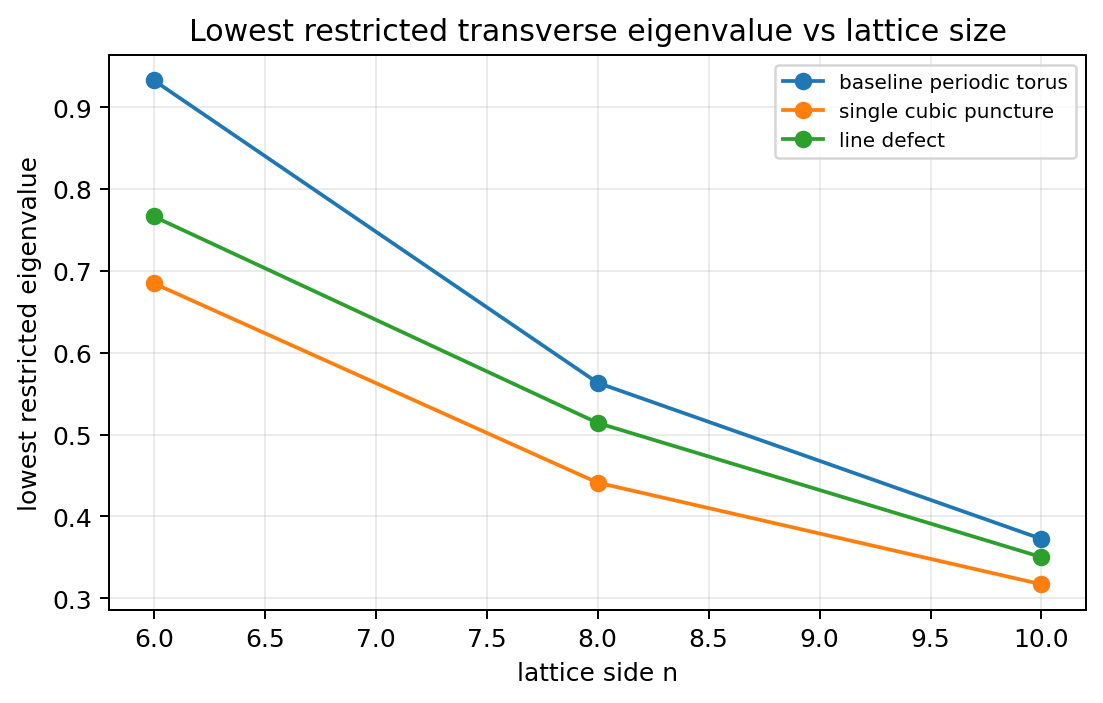
\includegraphics[width=0.32\linewidth]{../plots/20260310_130326_restricted_eigenvalue_vs_n.png}
\caption{Committed plots from \texttt{L1\_Defect\_Transverse\_Test\_v1}. Left: divergence--curl phase plot for the low edge spectrum. Center: restricted transverse spectrum in the three branches. Right: descent of the lowest restricted eigenvalue with lattice size.}
\label{fig:defect-test}
\end{figure}

The result of this first defect test is narrow but important: modifying the substrate weakens harmonic dominance and lowers the restricted transverse floor relative to the baseline torus. At this stage the experiment does not distinguish a continuum band from a defect-localized mode, but it establishes a descending low branch in the restricted operator.

\section{Transverse Scaling Test}
The committed scaling experiment \texttt{L1\_Transverse\_Scaling\_Test\_v1} extends the three branches to $n = 6, 8, 10, 12, 14, 16$ and measures both the lowest restricted eigenvalue and localization diagnostics. The fit
\begin{equation}
\lambda_{\min}(n) \approx a n^{-p}
\end{equation}
is applied branch by branch. The measured parameters are:
\begin{table}[t]
\centering
\begin{tabular}{lccc}
\toprule
Branch & $a$ & $p$ & $R^2$ \\
\midrule
Baseline torus & 26.7146 & 1.8621 & 0.9996 \\
Puncture & 11.7572 & 1.5781 & 0.9989 \\
Line defect & 16.8815 & 1.6983 & 0.9965 \\
\bottomrule
\end{tabular}
\caption{Power-law fits from \texttt{L1\_Transverse\_Scaling\_Test\_v1}. The exponents are below but near the $p=2$ window expected for a Laplacian-type continuum band on a finite domain.}
\label{tab:scaling-fits}
\end{table}

The localization metrics move in the same direction. For the puncture branch, the inverse participation ratio decreases from $0.006034$ at $n=6$ to $0.000183$ at $n=16$, while the near-defect norm fraction decreases from $0.547$ to $0.020$. For the line-defect branch, the same quantities decrease from $0.006203$ to $0.000533$ and from $0.513$ to $0.013$, respectively. The baseline branch also delocalizes with increasing size.

\begin{figure}[t]
\centering
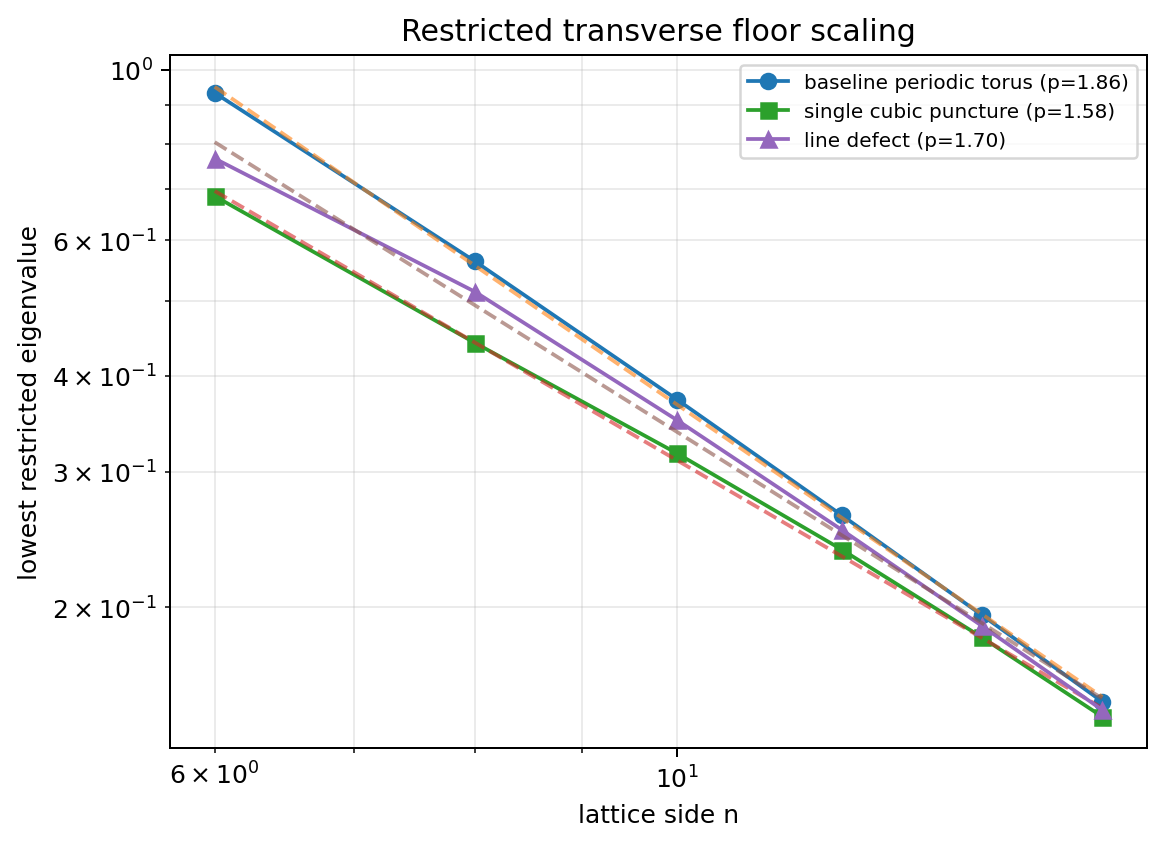
\includegraphics[width=0.32\linewidth]{../plots/20260310_132323_transverse_floor_scaling_loglog.png}
\hfill
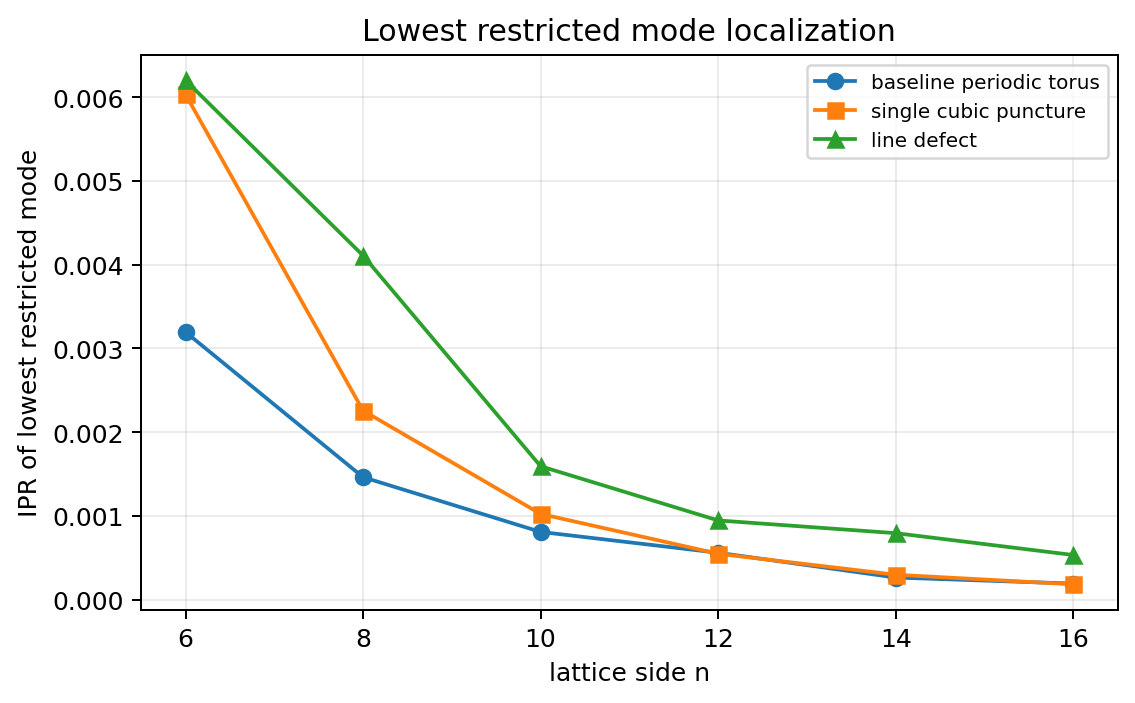
\includegraphics[width=0.32\linewidth]{../plots/20260310_132323_transverse_floor_ipr_vs_n.png}
\hfill
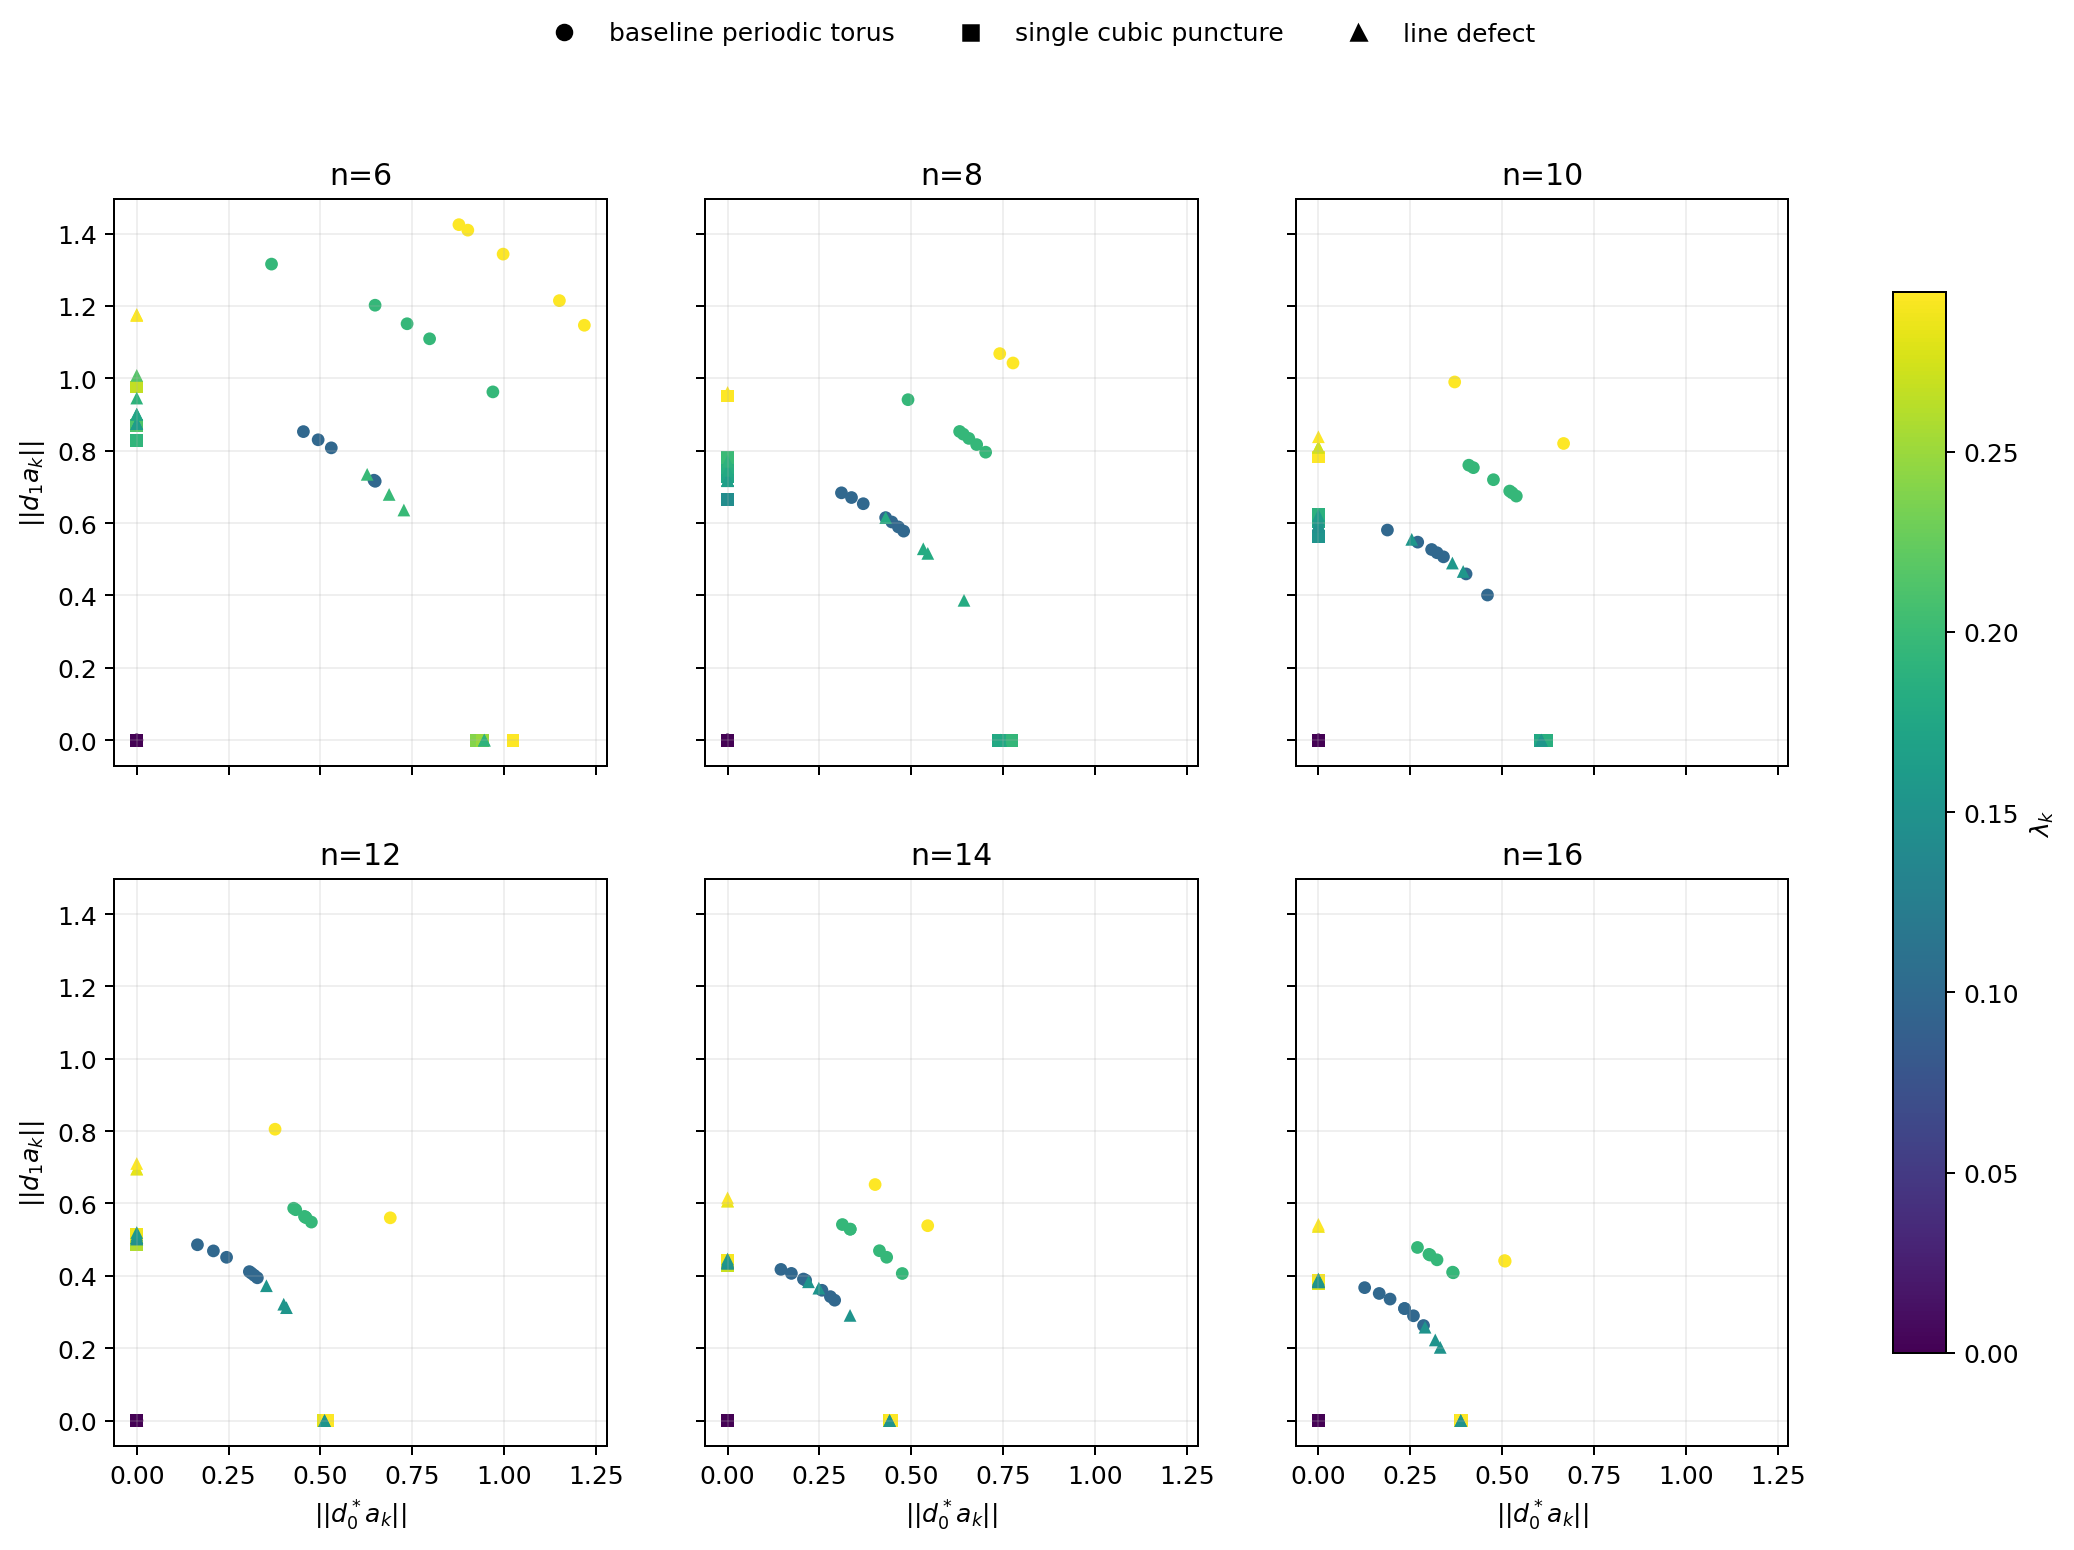
\includegraphics[width=0.32\linewidth]{../plots/20260310_132323_divergence_curl_phase_scaling.png}
\caption{Committed plots from \texttt{L1\_Transverse\_Scaling\_Test\_v1}. Left: log--log scaling of the lowest restricted eigenvalue. Center: IPR of the lowest restricted mode versus lattice size. Right: divergence--curl phase structure across the scaling scan.}
\label{fig:scaling-test}
\end{figure}

Taken by itself, this experiment supports the bounded statement that the descending restricted floor behaves more like a continuum transverse-band candidate than a defect-pinned low mode in the tested range.

\section{Transverse Band Test (Flux Tube)}
The committed band test \texttt{L1\_Transverse\_Band\_Test\_v1} adds a fourth branch while keeping the operators unchanged:
\begin{enumerate}
\item baseline torus,
\item puncture,
\item line defect,
\item flux-tube defect.
\end{enumerate}
The flux tube modifies holonomy while preserving lattice connectivity. For each branch and each $n = 6, 8, 10, 12, 14, 16$, the first twenty restricted transverse eigenvalues are computed and rescaled as $n^2 \lambda_k$.

The key diagnostic is spectral collapse. The mean relative spread of the first ten scaled modes is
\begin{equation}
0.073 \; (\text{baseline}),
\quad
0.086 \; (\text{puncture}),
\quad
0.070 \; (\text{line defect}),
\quad
0.053 \; (\text{flux tube}).
\end{equation}
These values show that several low restricted modes, not only the first one, are already clustering into a common envelope across lattice sizes.

The localization diagnostics remain consistent with that picture. For the flux-tube branch, the lowest restricted-mode IPR decreases from $0.004831$ at $n=6$ to $0.000187$ at $n=16$, while the near-tube norm fraction decreases from $0.340$ to $0.058$. The lowest restricted mode remains numerically transverse throughout the scan: $\|d_0^* a\|$ stays at the level of $10^{-16}$ while $\|d_1 a\|$ remains finite.

\begin{table}[t]
\centering
\begin{tabular}{lcccc}
\toprule
Branch & $p$ & Spread of first 10 scaled modes & IPR at $n=6$ & IPR at $n=16$ \\
\midrule
Baseline torus & 1.8621 & 0.0731 & 0.002718 & 0.000235 \\
Puncture & 1.5781 & 0.0860 & 0.004395 & 0.000133 \\
Line defect & 1.6983 & 0.0705 & 0.005238 & 0.000329 \\
Flux tube & 1.6956 & 0.0534 & 0.004831 & 0.000187 \\
\bottomrule
\end{tabular}
\caption{Summary metrics from \texttt{L1\_Transverse\_Band\_Test\_v1}. The restricted transverse band shows partial $n^2$ collapse together with strong delocalization in all four branches.}
\label{tab:band-metrics}
\end{table}

\begin{figure}[p]
\centering
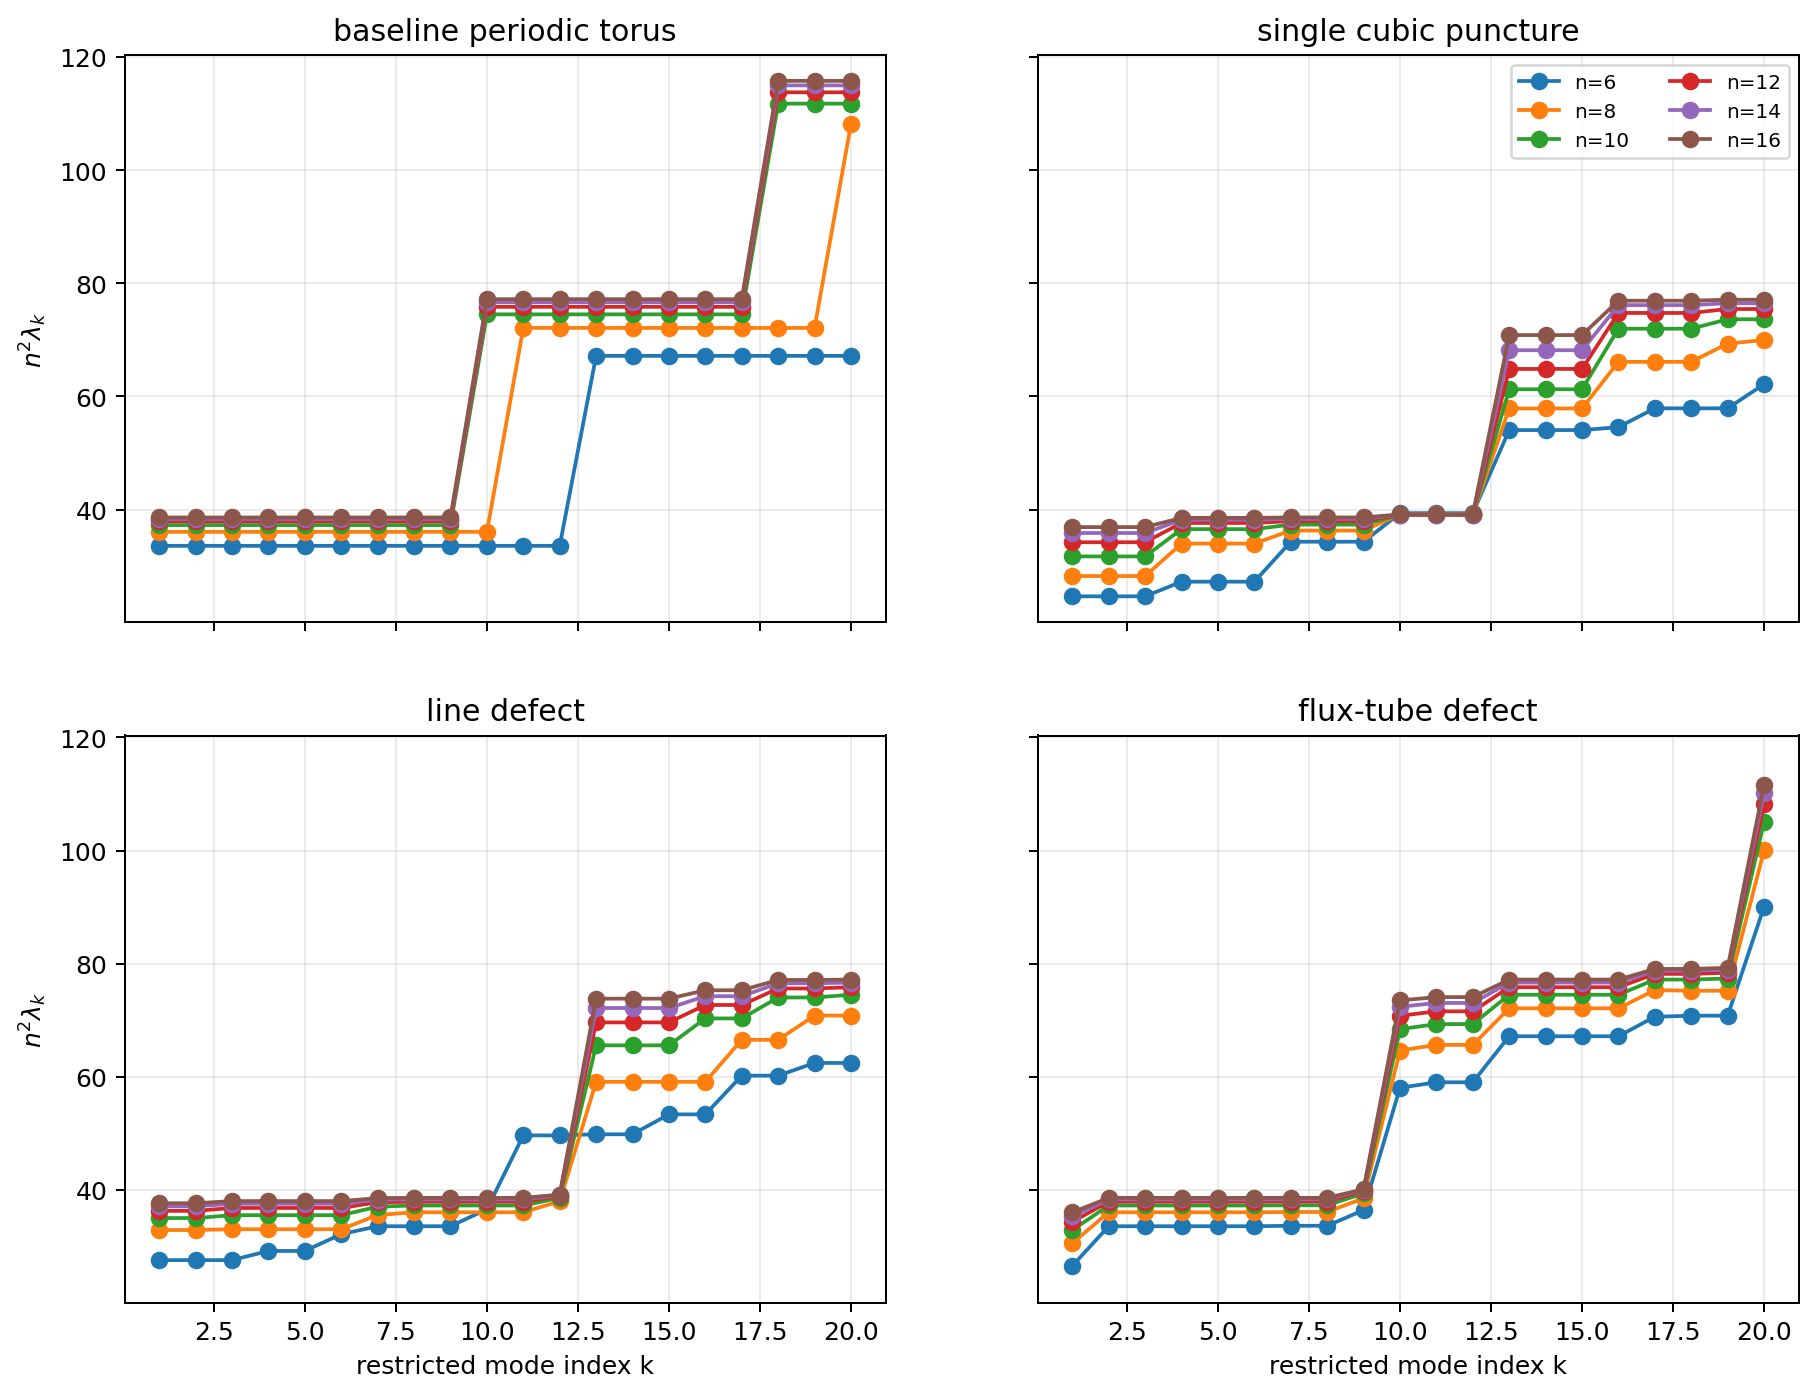
\includegraphics[width=0.48\linewidth]{../plots/20260310_133322_transverse_band_collapse.png}
\hfill
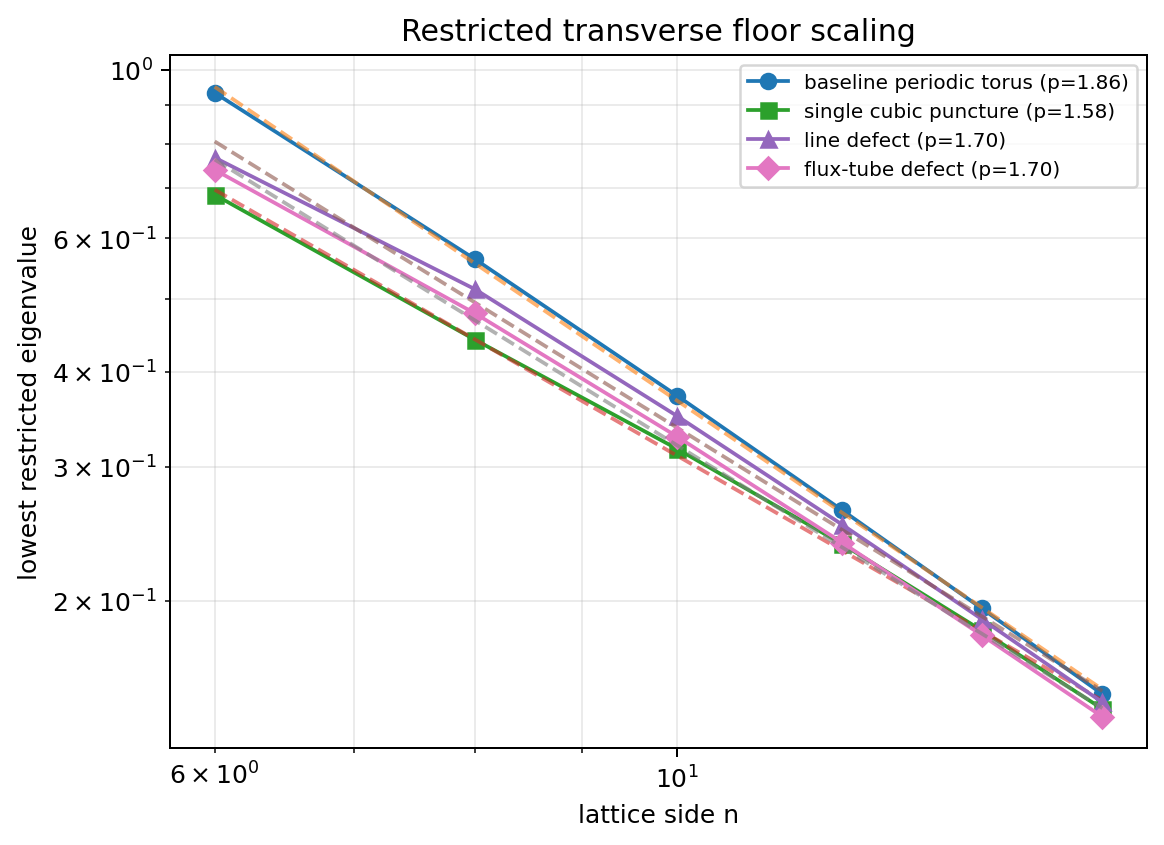
\includegraphics[width=0.48\linewidth]{../plots/20260310_133322_transverse_floor_vs_n.png}\\[1em]
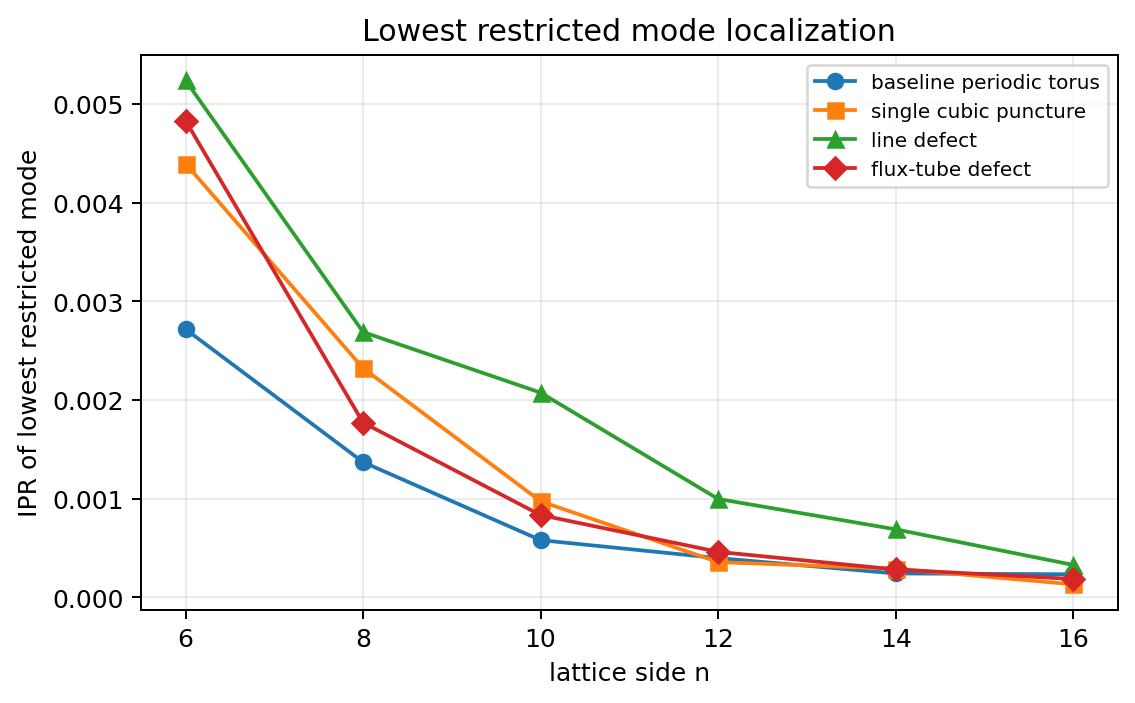
\includegraphics[width=0.48\linewidth]{../plots/20260310_133322_transverse_ipr_vs_n.png}
\hfill
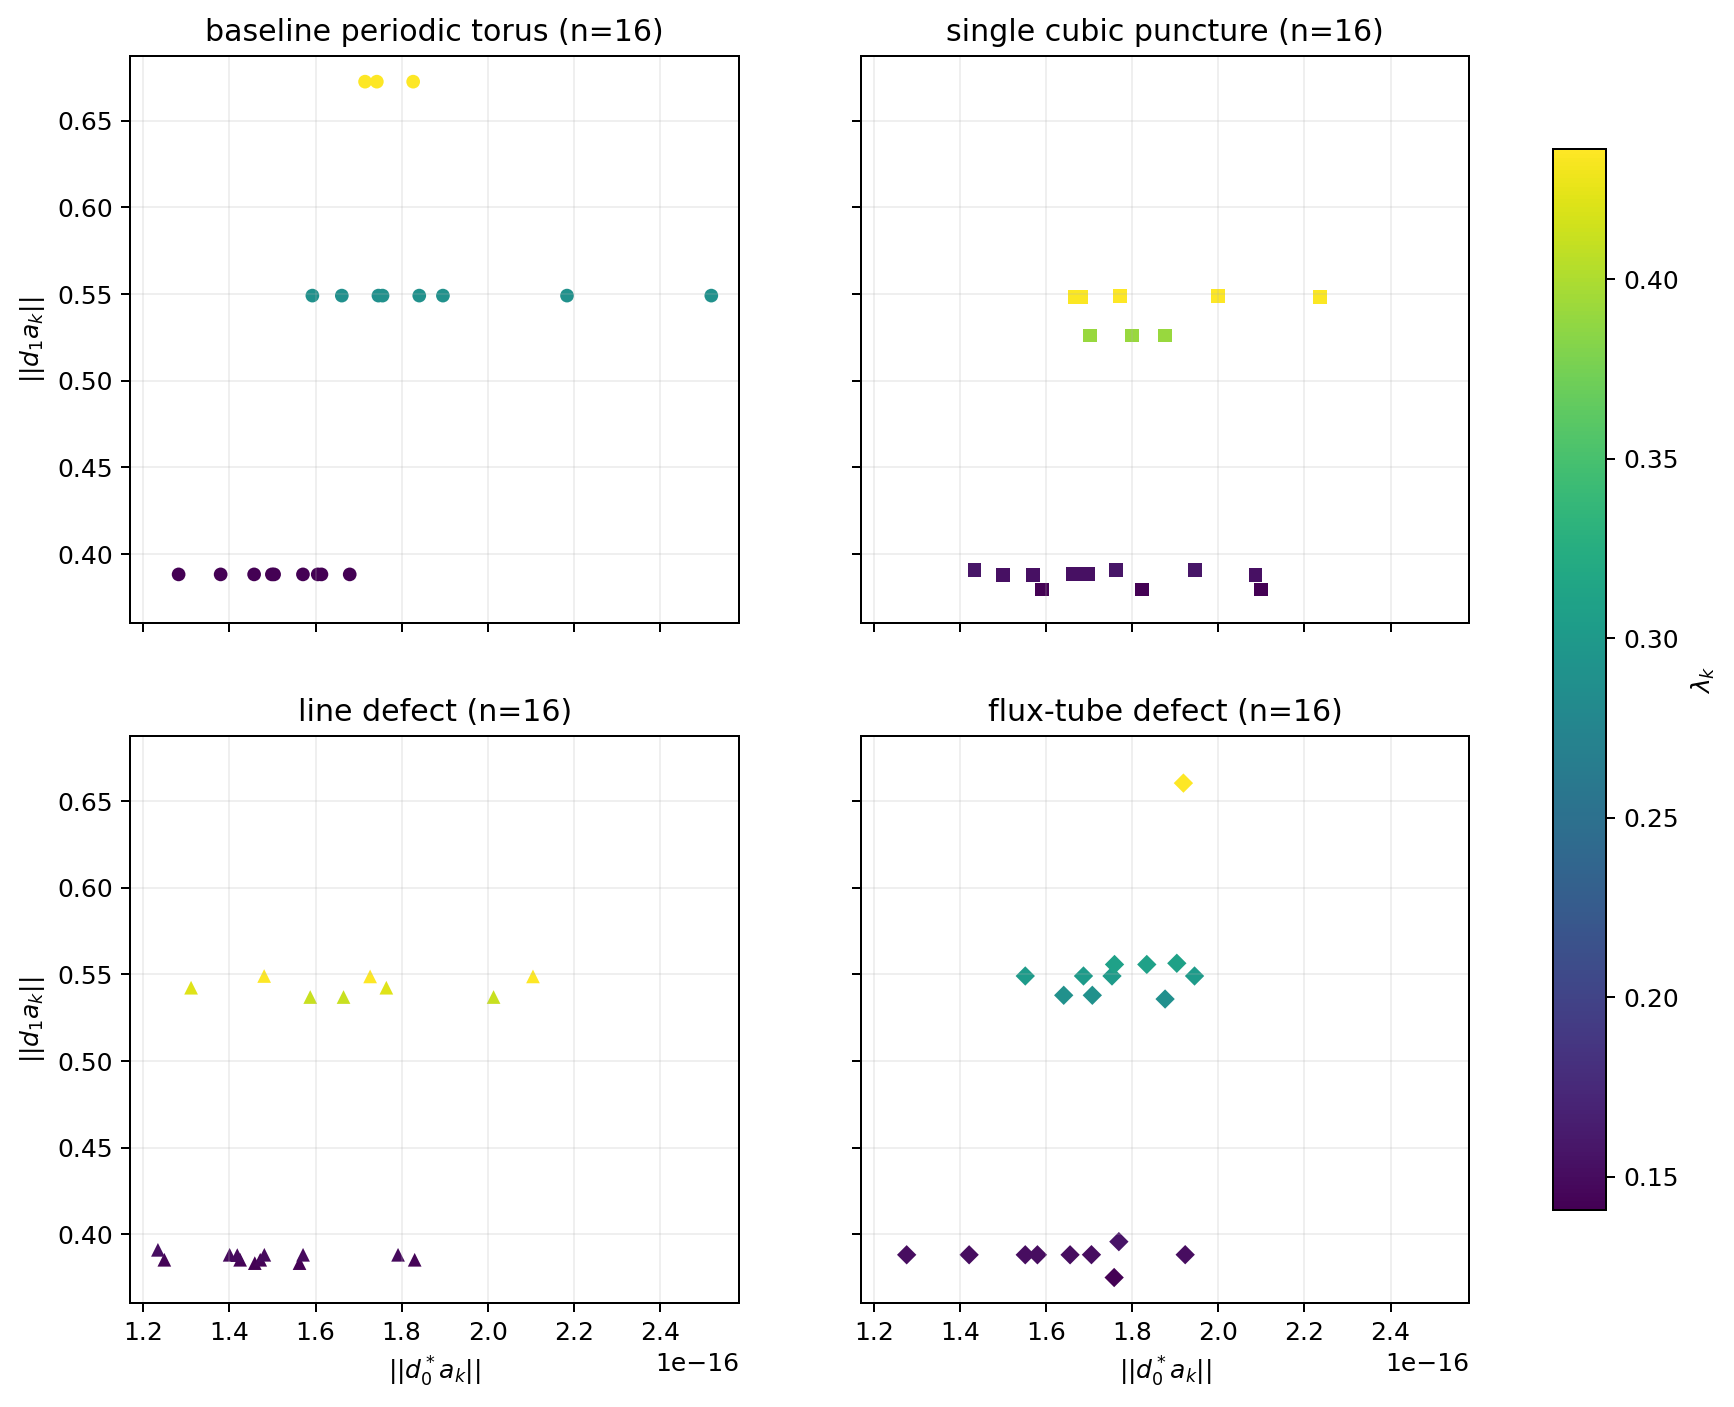
\includegraphics[width=0.48\linewidth]{../plots/20260310_133322_divergence_curl_phase_band.png}\\[1em]
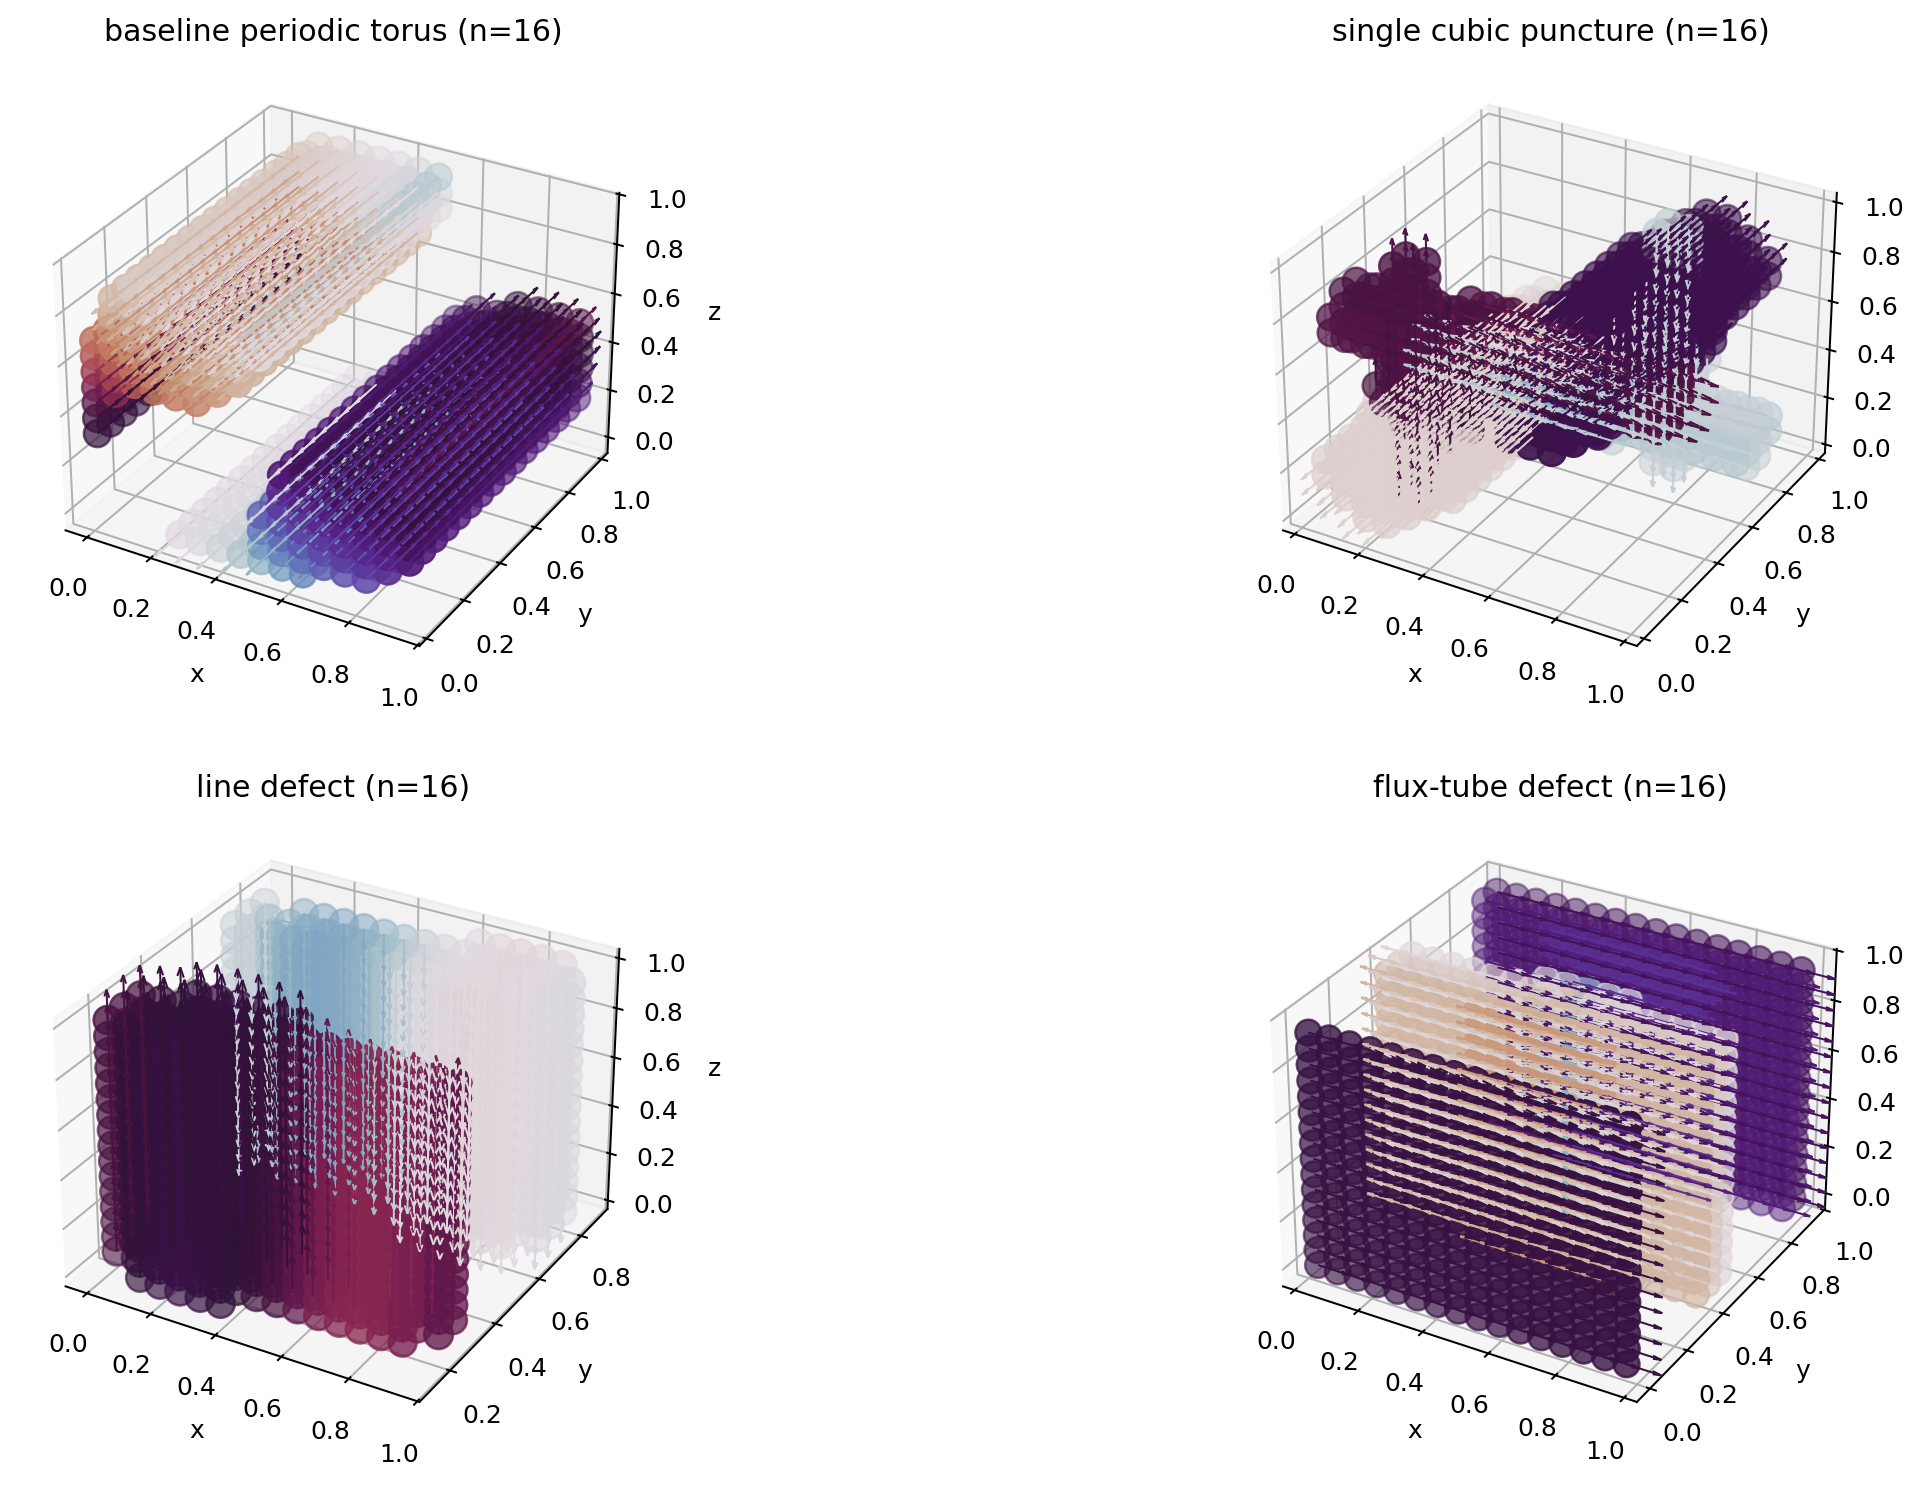
\includegraphics[width=0.65\linewidth]{../plots/20260310_133322_transverse_mode_profiles.png}
\caption{Committed plots from \texttt{L1\_Transverse\_Band\_Test\_v1}. Top left: $n^2\lambda_k$ versus mode index for the first twenty restricted transverse modes. Top right: lowest restricted eigenvalue versus $n$. Bottom left: IPR of the lowest restricted mode versus $n$. Bottom right: divergence--curl phase plot for the band scan. Bottom center: representative spatial profiles of the lowest restricted transverse modes.}
\label{fig:band-test}
\end{figure}

Within the tested range, the combined diagnostics support the statement that the restricted transverse sector is organizing as a stable low spectral band rather than only producing a single descending impurity mode.

\section{Interpretation Boundary}
The committed experiments provide operator-level numerical evidence for a low transverse spectral band consistent with continuum scaling in the tested range. That statement is bounded by design. The results do not establish Maxwell dynamics, gauge theory, or physical photon modes. No independent gauge-field action, continuum field normalization, or dynamical photon observable is introduced in the present repository state.

What is supported is narrower and more concrete:
\begin{enumerate}
\item the Gaussian interaction kernel induces a scalar operator with a Laplacian continuum limit,
\item the same substrate supports an edge or Hodge operator with a non-scalar restricted sector,
\item after exact and harmonic components are removed, the low restricted spectrum descends, delocalizes, and shows partial continuum-band collapse.
\end{enumerate}
This is the appropriate interpretation boundary for the current numerical record.

\section{Conclusion}
The current HAOS-IIP repository supports the following operator architecture at the numerical level:
\begin{equation}
\text{single kernel substrate}
\to
\text{scalar Laplacian sector}
\to
\text{edge/Hodge sector}
\to
\text{restricted transverse band candidate}.
\end{equation}
The scalar branch is established through the kernel-to-Laplacian convergence experiment. The edge branch is established through the Hodge construction, the open-versus-periodic diagnostic, and the defect-controlled restricted-sector scans. The most recent band test shows a descending, delocalizing, partially collapsing low restricted spectrum across baseline, puncture, line-defect, and flux-tube branches.

The next numerical steps are straightforward and do not require new operator definitions: larger lattices to test the approach toward the expected asymptotic scaling, spectral-density measurements of the restricted band, and direct comparison with the continuum vector Laplacian. For the present paper, however, the main result is already clear: the committed repository state contains operator-level numerical evidence that a single kernel-defined discrete substrate supports both a scalar Laplacian sector and a low transverse edge-sector band candidate.

\section*{Project Resources}
Project website: \url{https://tomislav-rupic.com/}

Code repository: \url{https://github.com/tomislavrupic}

Archived release (Zenodo DOI): \url{https://doi.org/10.5281/zenodo.18938323}

\end{document}
